\documentclass[11pt,letterpaper]{article}
\usepackage[margin=.7in]{geometry}
\usepackage{amsmath,amssymb,graphicx,booktabs,pdflscape,caption,microtype,xcolor,hyperref}
\hypersetup{colorlinks=true,urlcolor=blue!55!black,linkcolor=blue!55!black,citecolor=blue!55!black,pdftitle={HPS-GPR v5.5.3: The 92 MeV line, combined profiles and exposure checks}}
\setlength{\parindent}{0pt}\setlength{\parskip}{6pt}\captionsetup{font=small,labelfont=bf}
\begin{document}
\begin{landscape}
{\Large\bfseries HPS-GPR v5.5.3: the 92 MeV line}\par
12 September 2026 \quad | \quad Combined rates, centroids, resolutions and smaller-sample checks
\begin{center}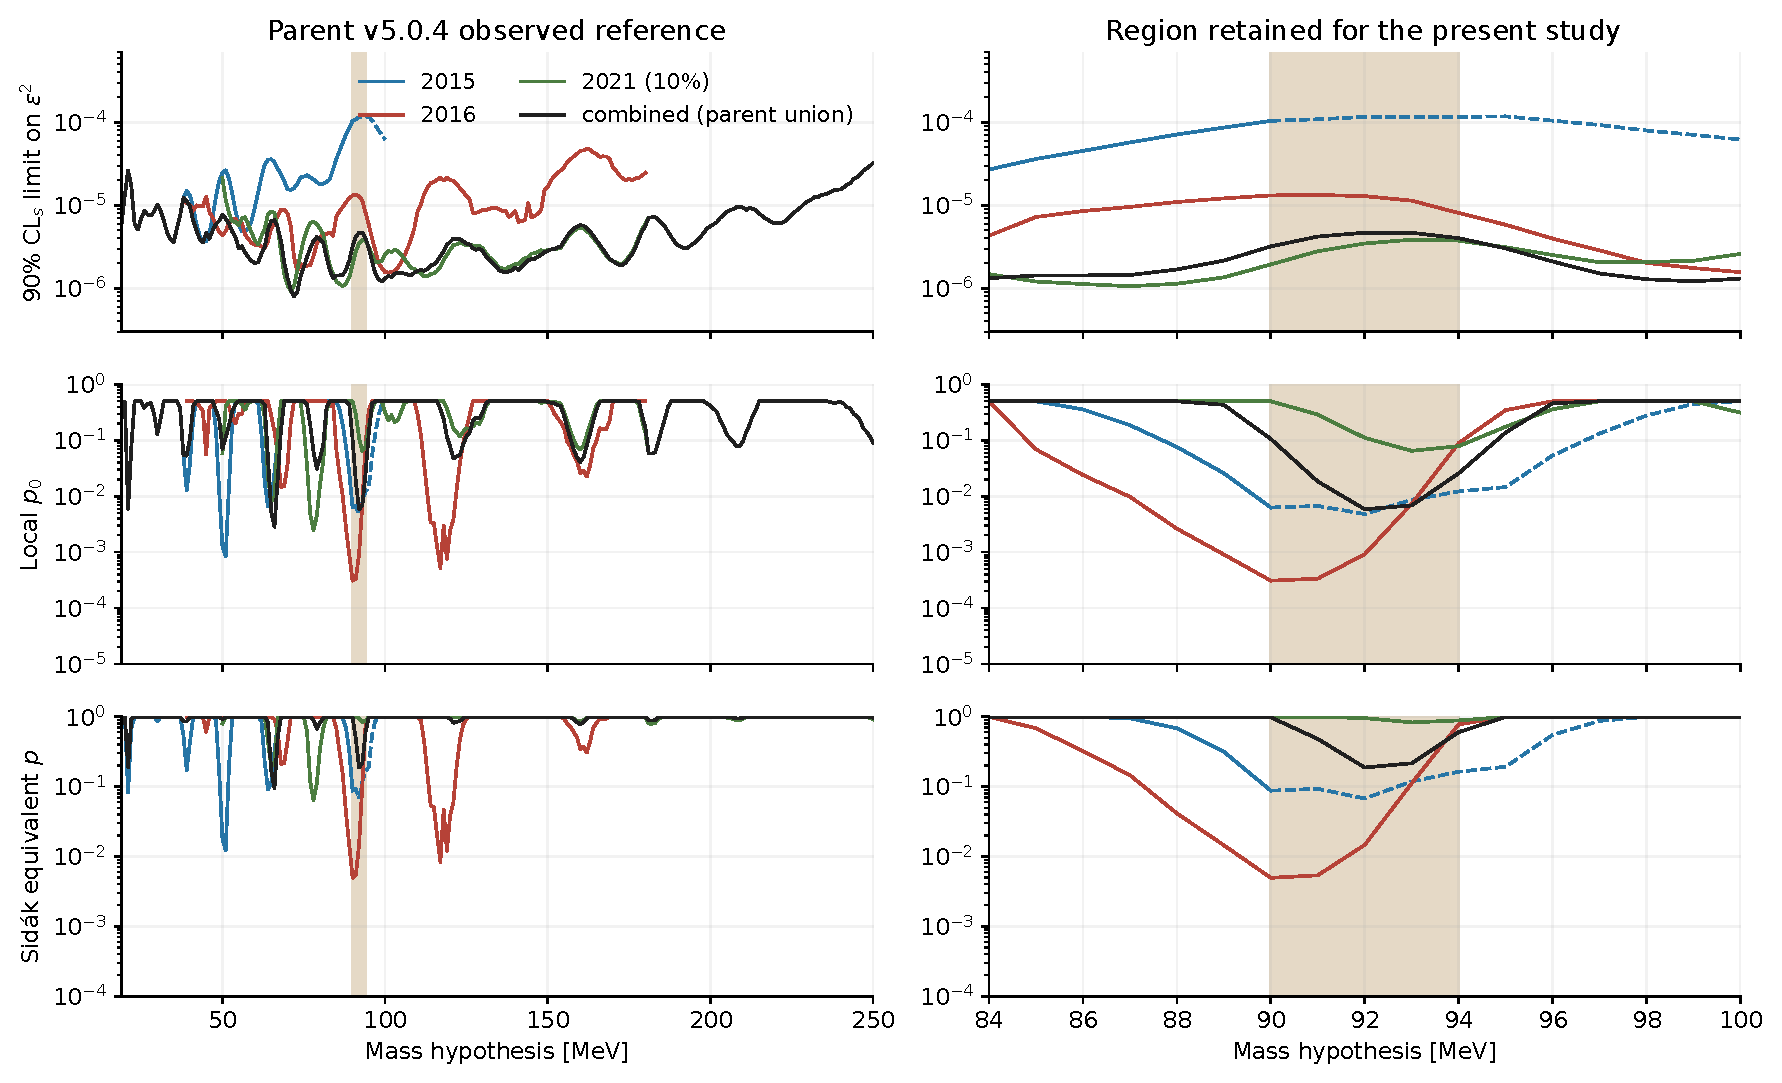
\includegraphics[height=5.35in]{../figures/opening_limits_probabilities.pdf}\end{center}
\captionof{figure}{The unchanged v5.0.4 limits, local asymptotic $p_0$, and Sid\'ak-equivalent probabilities are the reference being combined. Shading marks 90--94 MeV; dashed 2015 segments denote its exploratory extension. Black is the parent union, whose active campaigns change with mass. The heuristic mapping is $p_{\rm Sidak}=1-(1-p_0)^{N_{\rm eff}}$, using $N_{\rm eff}=14.521,16.062,26.402$ for the campaigns and 35.381 for the union. These are not trials factors calibrated for the new fits.}
\end{landscape}

\clearpage
\section*{What combined significance follows from the rate model?}
Allowing different campaign rates removes much of the common-coupling mismatch. On the exact v5.5.0 windows, the common-coupling likelihood root is 2.520, while its fitted energy response gives 4.213. The latter is a raw $\sqrt{Q_0}$, not automatically a local Gaussian significance: the energy exponent was fitted from these same events.

For the common fixed experiment defined below, the corresponding roots are 2.447 and 4.180. A local predictive-Gaussian reference that includes the exponent search gives $p_G=(6.81\pm0.14)\times10^{-5}$, or $Z_G=3.815$. Letting a common centroid vary over 90--94 MeV gives a slightly larger root, 4.206, but $p_G=(2.090\pm0.033)\times10^{-4}$ and $Z_G=3.528$. The added search freedom outweighs the small fit improvement.

\begin{center}\small\begin{tabular}{lrrrr}\toprule
Model & $\sqrt{Q_0}$ & $\widehat\beta$ & Reference $p_G$ & $Z_G$\\\midrule
92; scaled & 4.180 & -2.987 & $6.81\times10^{-5}$ & 3.815\\
Shared mass; scaled & 4.206 & -3.043 & $2.09\times10^{-4}$ & 3.528\\
Separate masses; scaled & 4.500 & -2.883 & $2.43\times10^{-4}$ & 3.488 $\dagger$\\
92; width nuisance & 4.423 & -3.072 & $7.18\times10^{-5}$ & 3.802 $\dagger$\\
Shared mass; width nuisance & 4.428 & -3.044 & $2.55\times10^{-4}$ & 3.475 $\dagger$\\
Separate masses; width nuisance & 4.598 & -2.878 & $2.88\times10^{-4}$ & 3.443 $\dagger$\\
92; MC reference & 4.388 & -3.109 & $2.88\times10^{-5}$ & 4.022\\
\bottomrule\end{tabular}
\end{center}
All rows fit the energy exponent on $[-6,6]$. A dagger denotes a \emph{broader independent-amplitude reference evaluated at the energy-model statistic}, not the energy model's own probability. Those entries indicate a conservative comparison family on the sampled shape grid; they are not rigorous bounds on the continuous family. Thus the most flexible fit has raw root 4.598 and reference-envelope $Z_G=3.443$, without establishing a model-specific $4.598\sigma$ result. The quoted errors above are Monte Carlo errors of the reference calculation, not background-model uncertainties. All references remain local to the specified hypothesis or 90--94 MeV search, not globally calibrated evidence.

\section*{A common experiment for every comparison}
The signal model is
\[
 \lambda_i=b_i+L_i\theta_i+\mu K_i(m_i,\sigma_i)
       (E_i/2.30\,\mathrm{GeV})^\beta,\qquad \mu\geq0.
\]
Here $Q_0=2(\mathrm{NLL}_0-\mathrm{NLL}_{\rm best})$ includes the stated constraints; each GP nuisance vector has penalty $\theta_i^T\theta_i/2$.
The energies are 1.056, 2.30 and 3.74 GeV. $K_i$ includes the inherited radiative fraction and a density conversion evaluated once using the MC reference at 92 MeV; its bin-integrated Gaussian shape can vary. The extra power is a residual accepted-rate parametrization after that normalization, not coupling running or a second production factor~\cite{hps,bjorken}.

Every new model uses the same per-campaign bins and GP constraint: the union of means 90--94 MeV padded by $2.25$ fully scaled resolutions. The windows are 79.19--104.81, 81.48--102.52 and 84.49--99.51 MeV, containing 102, 84 and 24 bins. Kernel parameters remain at 92 MeV (the frozen 90 MeV state for 2015); sideband support is unchanged. Signal fractions outside the fit windows are retained rather than renormalized away. Changing the window accounts for most of the small difference from the historical roots. No likelihoods from different experiments or overlapping mass windows are pooled.

\clearpage
\begin{landscape}
\section*{The common-coupling interpretation revisited}
\begin{center}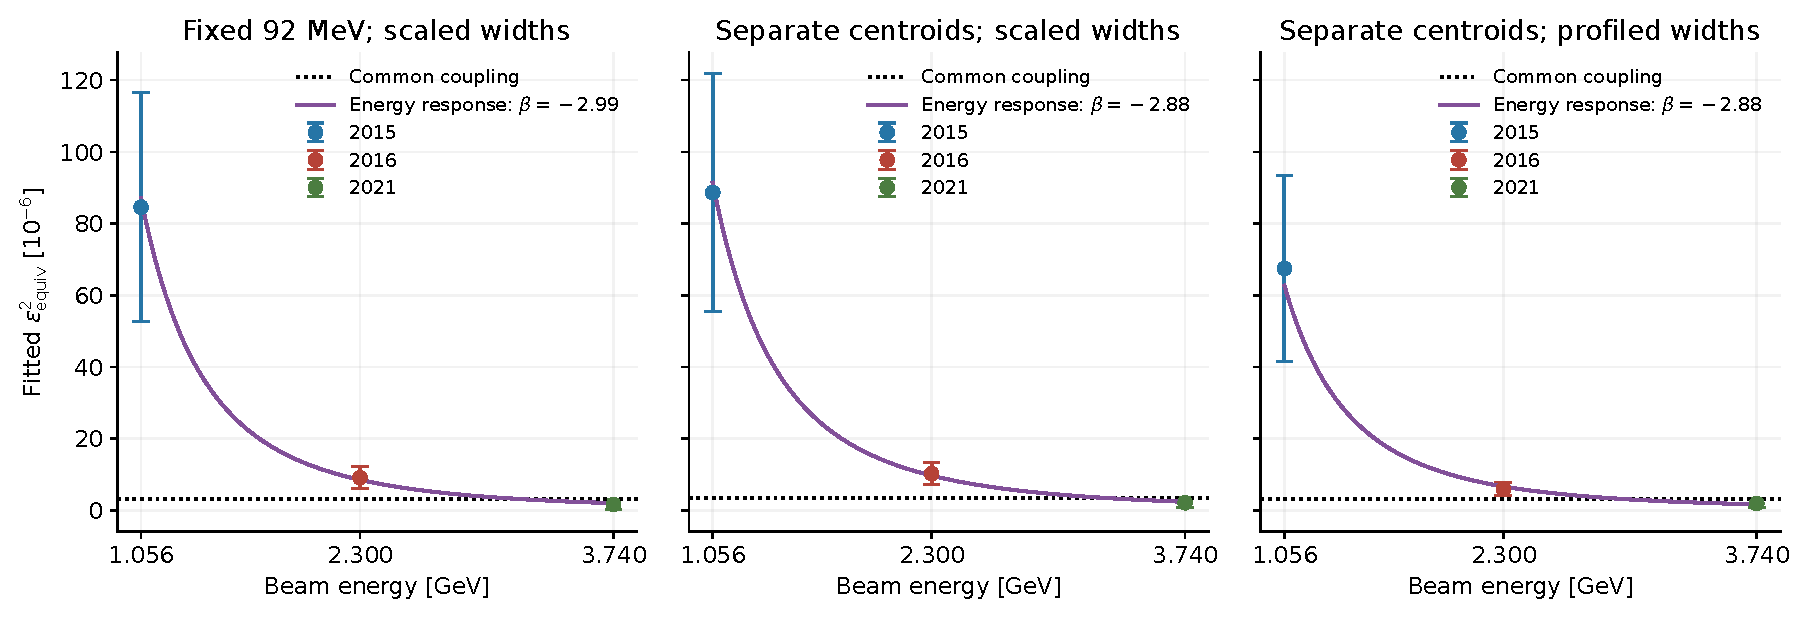
\includegraphics[width=.99\linewidth]{../figures/rate_interpretation_comparison.pdf}\end{center}
\captionof{figure}{A counterpart of v5.5.0 Figure 2. Points are independently fitted nonnegative campaign amplitudes, with curvature errors conditional on their fitted shapes. Dotted lines show the common-coupling normalization; purple curves show the fitted energy response. Each model profiles its own allowed shapes on the same data and background constraint. Thus the floating-shape points and curve need not use identical centroids or widths. These are equivalent template normalizations, not measured particle couplings.}

At fixed 92 MeV with scaled widths, fitting the energy response increases $Q_0$ from 5.986 to 17.474, leaving only 0.105 below three independently fitted positive rates. This is the sense in which the common-coupling suppression is removed. The fitted exponent is $-2.987$ in this fixed experiment, close to the original $-2.904$. A law fixed independently of these events would permit the usual one-amplitude reference, subject to its background assumptions. Freezing a slope after fitting these same events does not erase that adaptation~\cite{cowan,gross}.

Independent rates provide a useful limiting comparison: at a fixed shape their Gaussian-reference statistic has the mixture $\tfrac18\chi^2_0+\tfrac38\chi^2_1+\tfrac38\chi^2_2+\tfrac18\chi^2_3$. Its tail, rather than $\Phi(-\sqrt{Q_0})$, accounts for the three nonnegative amplitudes. Rate flexibility can improve the fit substantially without giving the entire likelihood gain the interpretation of extra significance.
\end{landscape}

\clearpage
\begin{landscape}
\section*{Where the fits put the centroids and resolutions}
\begin{center}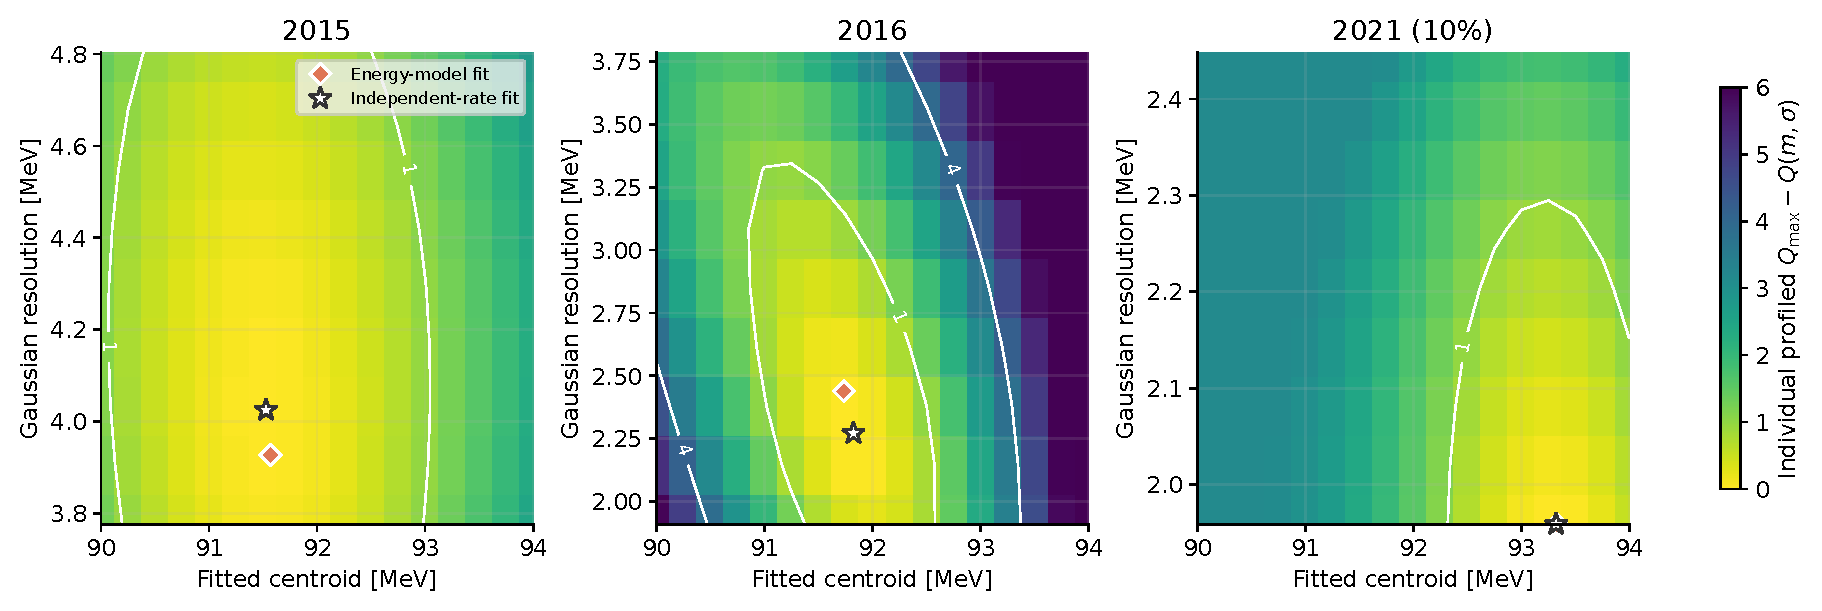
\includegraphics[width=.99\linewidth]{../figures/centroid_resolution_profiles.pdf}\end{center}
\captionof{figure}{Individual amplitude-profiled shape surfaces with the MC-centered penalty. Colors and contours give differences in penalized $Q_0$; contours at 1 and 4 are descriptive. Diamonds mark the energy-model solution and stars independent rates. The lower and upper edges are MC-reference and scaled widths; 2021 reaches the lower edge.}
\begin{center}\small\begin{tabular}{lrrrrr}\toprule
Dataset & Centroid [MeV] & $\sigma_{\rm MC}$ & Fitted $\sigma$ & Scaled $\sigma$ & Fitted $t$\\\midrule
2015 & 91.567 & 3.777 & 3.928 & 4.804 & 0.147\\
2016 & 91.735 & 1.909 & 2.439 & 3.788 & 0.282\\
2021 & 93.327 & 1.959 & 1.959 & 2.449 & 0.000\\
\bottomrule\end{tabular}
\end{center}
All widths in the table are in MeV. The main width model follows v5.3:
\[
 \sigma_i=\sigma_{{\rm MC},i}+t_i(\sigma_{{\rm scaled},i}-\sigma_{{\rm MC},i}),
 \quad 0\leq t_i\leq1,\qquad -\log C_t=\tfrac12\sum_i t_i^2.
\]
This constraint is assumed, not a measured calibration likelihood. The 2015 MC reference is derived from a correction ratio; the 2021 reference precedes the additional TC scaling and need not be entirely unsmeared MC. No width falls below its reference. The fitted centroids span 1.760 MeV. Under a physical-line hypothesis these are reconstruction offsets, not different pole masses.

A bounded-flat control instead gives widths 4.804, 2.701 and 1.959 MeV, with raw root 4.645. The sizable 2015 width change shows sensitivity to the assumed constraint. Fixed scaled-width controls have no width penalty; the penalized family is nested above its fixed-MC member, but is not an ordinary unpenalized enlargement of the scaled-width control.
\end{landscape}

\clearpage
\begin{landscape}
\section*{Fit improvement versus local reference probabilities}
\begin{center}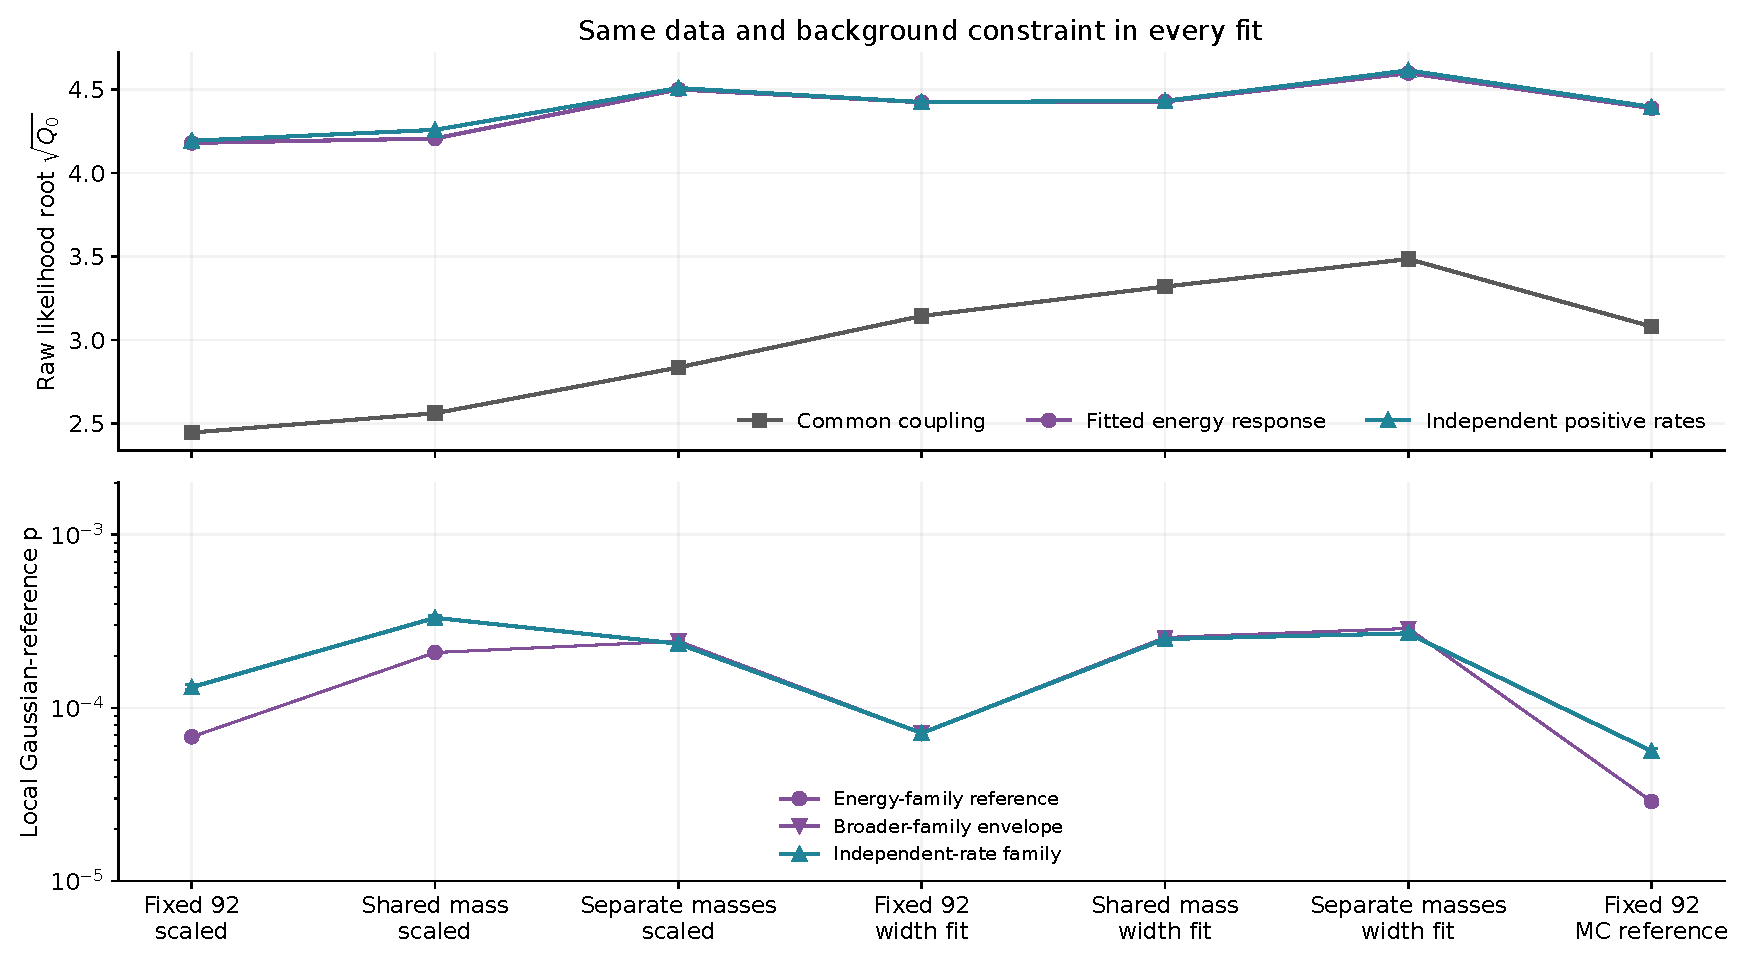
\includegraphics[height=4.6in]{../figures/likelihood_and_local_reference_comparison.pdf}\end{center}
\captionof{figure}{Top: exact conditional Poisson/Gaussian likelihood roots for three rate models. Bottom: predictive-Gaussian reference probabilities, with Monte Carlo error bars. Purple circles use the energy family itself; purple downward triangles use its broader independent-amplitude reference envelope. Blue triangles use independent rates. Lines guide the eye across distinct hypotheses, not nested steps in one scan. The final point is the fixed-MC control.}

The reference uses $V_i=\operatorname{diag}(\widehat\lambda_{0,i})+L_iL_i^T$, retaining the GP auxiliary contribution. It is not a Poisson-only null with the auxiliary measurement held fixed. The assumed width penalty is kept fixed. A shared 100,000-draw importance sample supplies finite-grid shape references; normal and three-amplitude mixture checks pass, Monte Carlo relative errors are at most 2.61\%, and grid-thinning changes the original reference tails by at most 2.48\%. The shared-mass energy test refines every detected exponent basin and has 1.40\% mean-grid sensitivity. These checks do not calibrate the original mass selection, detector modeling or direct Poisson tails. The original Sid\'ak factors therefore remain reference plots only; they are not transferred to this expanded search.
\end{landscape}

\clearpage
\begin{landscape}
\section*{The observed residuals under the competing fits}
\begin{center}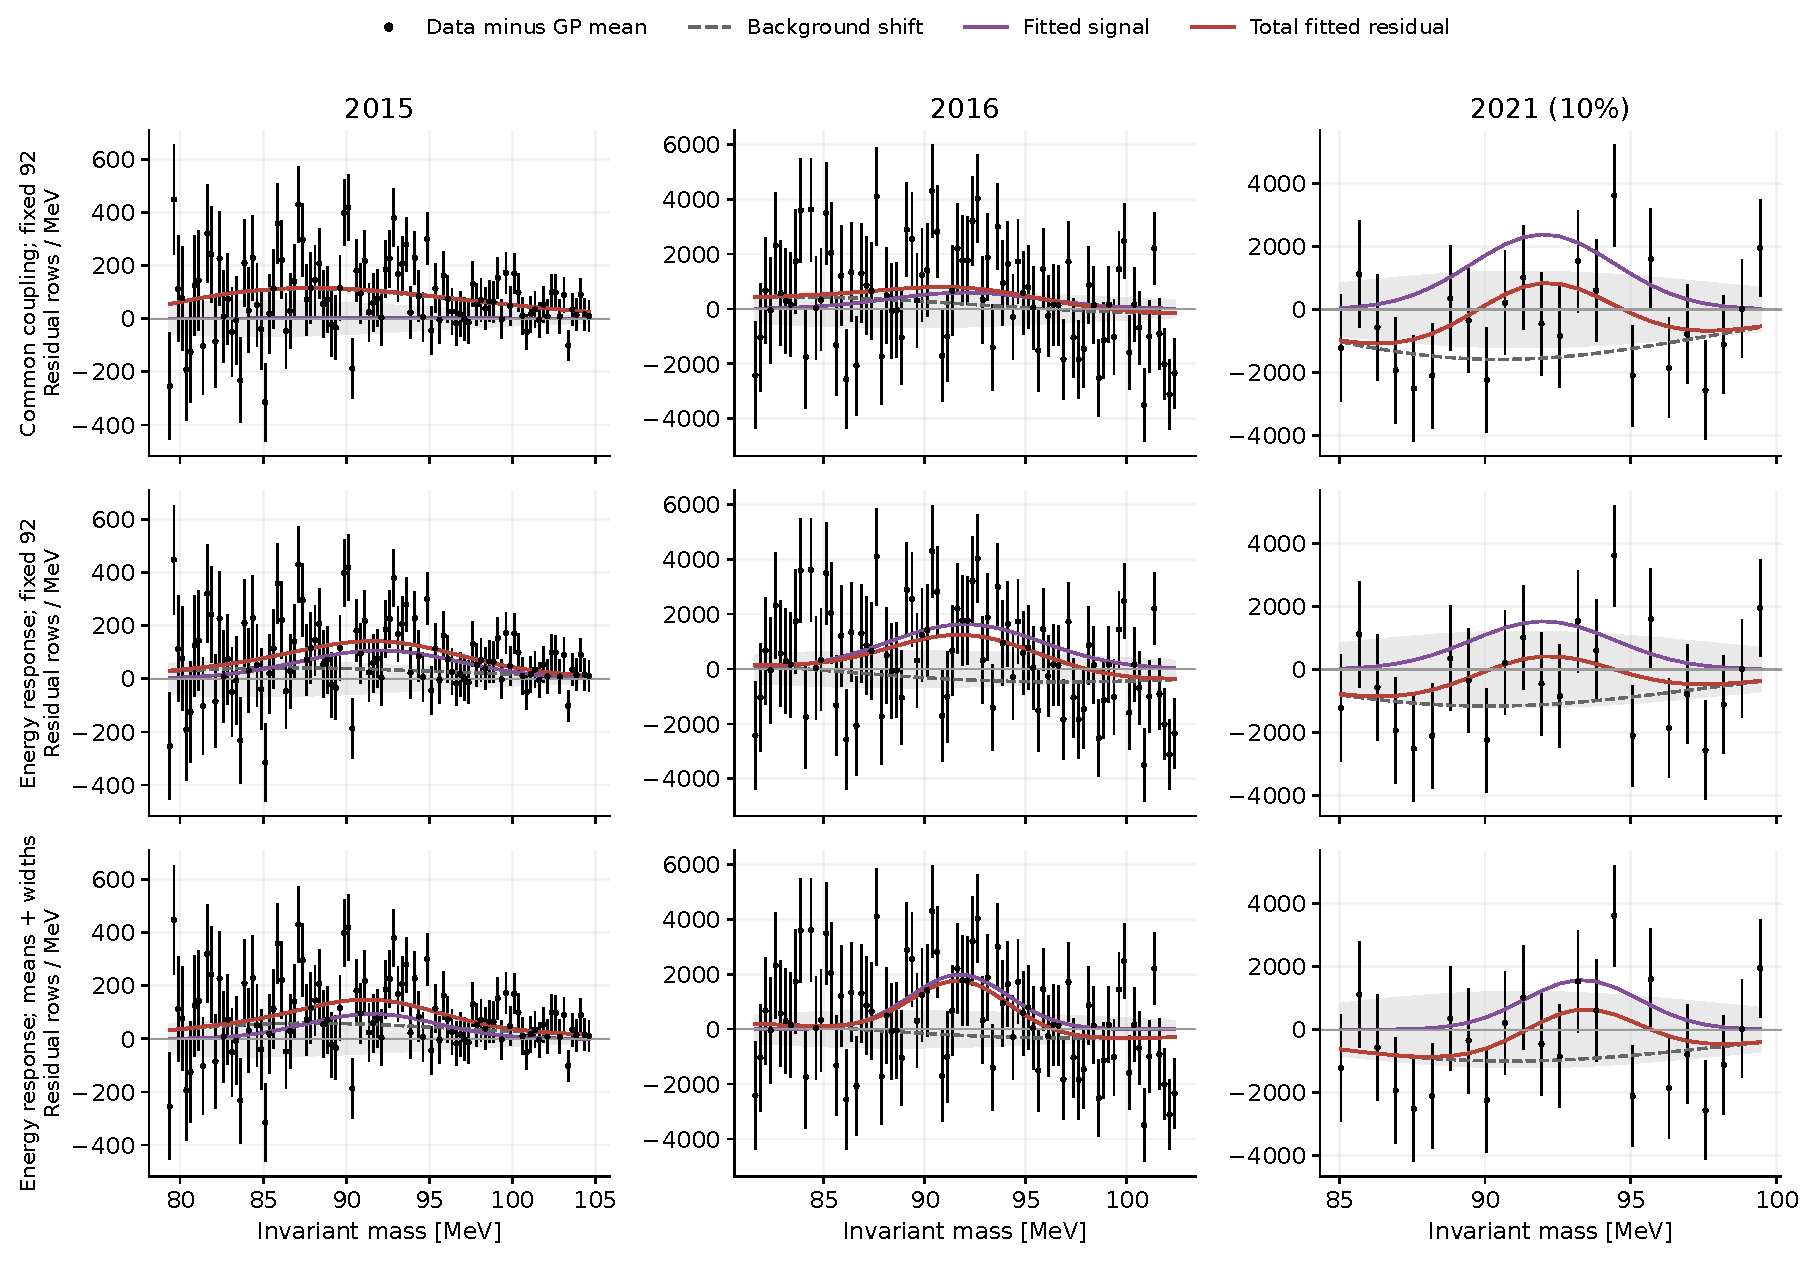
\includegraphics[height=5.65in]{../figures/extraction_model_comparison.pdf}\end{center}
\captionof{figure}{The same bins and GP mean appear in every row. Black points subtract that mean; error bars contain counting uncertainty only. Gray shading is the GP constraint standard deviation, the dashed line its fitted background adjustment, purple the signal, and red their sum. The top row imposes common coupling at 92 MeV; the middle fits the energy response at 92 MeV; the bottom also profiles separate centroids and bounded resolutions. Background adjustments remain visible rather than being attributed to the signal.}
\end{landscape}

\clearpage
\begin{landscape}
\section*{What the smaller samples show at 92 MeV}
\begin{center}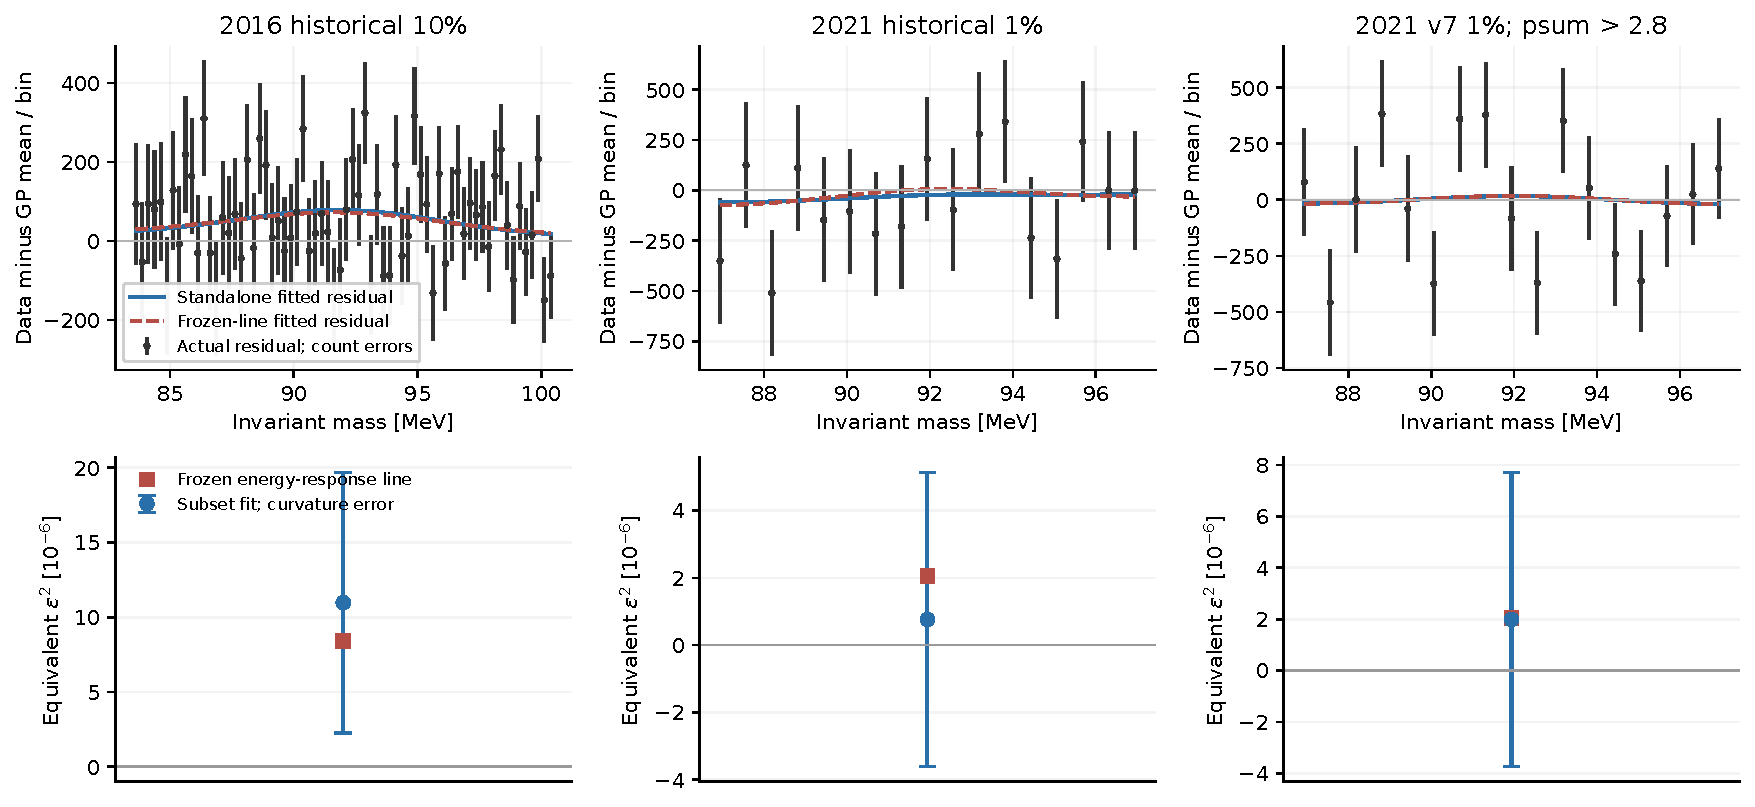
\includegraphics[height=3.65in]{../figures/subsets_actual_checks.pdf}\end{center}
\captionof{figure}{Actual smaller-sample histograms, with standalone and frozen-line fits. The line is the original v5.5.0 response at fixed 92 MeV, mapped through each histogram's density using inherited resolution and radiative-fraction proxies. These are not calibrated efficiency predictions. The lower panels compare equivalent amplitudes and local curvature errors.}
\begin{center}\small\begin{tabular}{lrrr}\toprule
Control sample & $\widehat\epsilon^2_{\rm equiv}$ [$10^{-6}$] & Signed $r$ & $D_{\rm line}$\\\midrule
2016 10\% & $10.98\pm8.72$ & 1.259 & 0.087\\
2021 historical 1\% & $0.76\pm4.38$ & 0.174 & 0.086\\
2021 v7 1\%; $p_{\rm sum}>2.8$ & $1.99\pm5.73$ & 0.347 & 0.000\\
\bottomrule\end{tabular}
\end{center}
All three fits are weakly positive and have limited precision. The 2016 10\% sample gives $r=1.259$. The two 2021 1\% variants give 0.174 and 0.347, so neither strongly tests the proposed line. $D_{\rm line}$ holds the predicted amplitude fixed and profiles the background; no parameter uncertainty is propagated.

The available 2021 files cannot be certified as the same prompt-TC selection as the native 10\% sample. The historical file's configuration refers to a different pair-momentum selection; the v7 histogram key labels $p_{\rm sum}>2.8$ GeV but contains no complete TC/run/event metadata. Their local count ratios to the native 10\% sample are 0.0885 and 0.0515, rather than a verified common exposure ratio. The 2016 ratio is 0.1023. Histograms alone do not establish event overlap or exact luminosity. These controls are not added as independent likelihood factors.
\end{landscape}

\clearpage
\begin{landscape}
\section*{A conditional view of 100\% 2021 statistics}
\begin{center}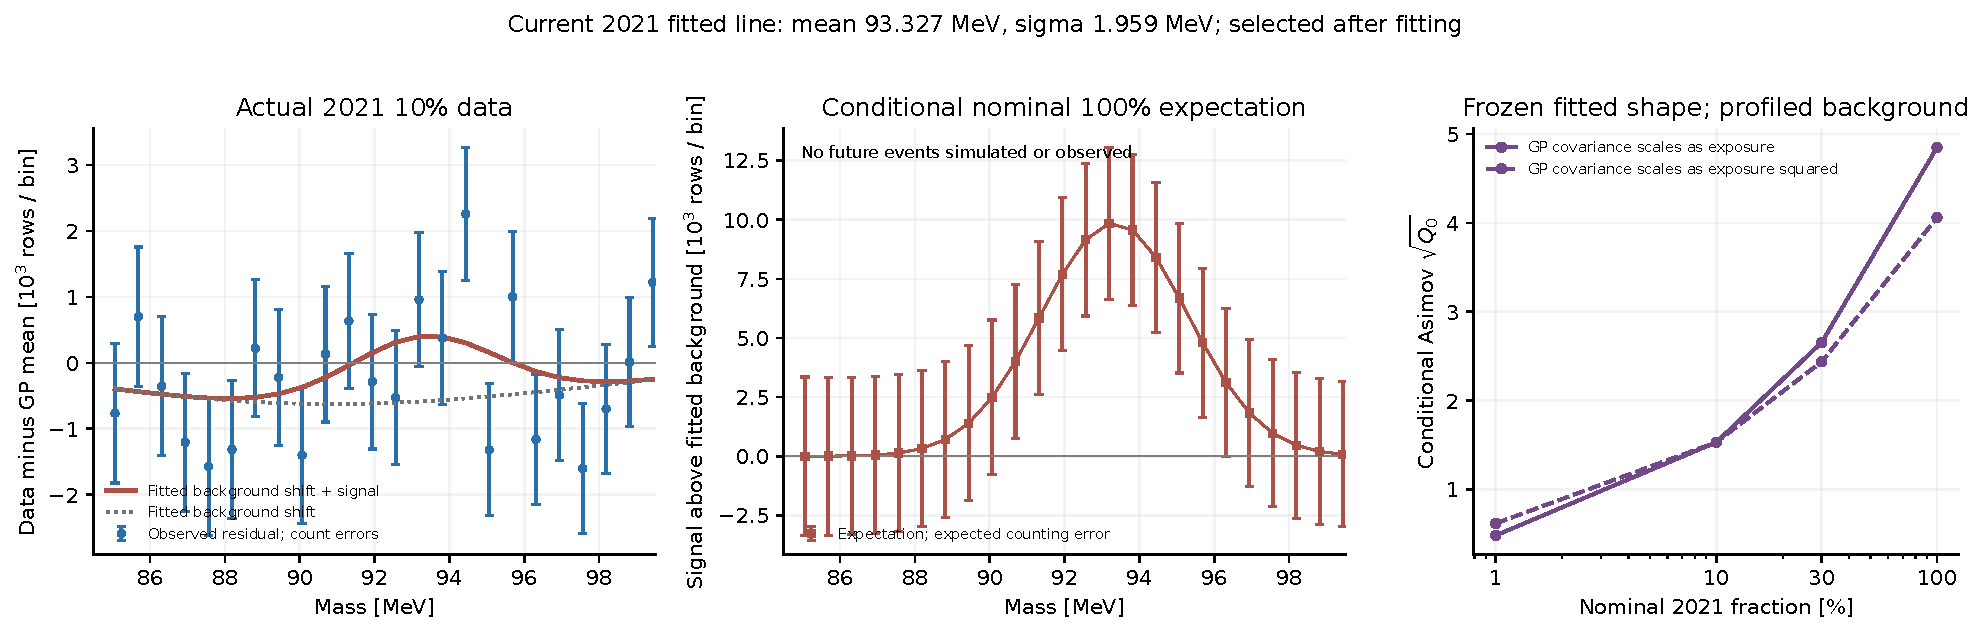
\includegraphics[width=.99\linewidth]{../figures/subsets_profiled_future_spectrum.pdf}\end{center}
\captionof{figure}{Left: actual 2021 10\% residuals and the current combined-model fit. Middle: the expected signal at nominal full exposure if that fitted line and background persist. The subtraction changes from the GP mean on the left to the fitted background in the middle, as labeled. Future points are expectations, with expected counting-error bars; no future data or random pseudo-data are shown. Right: exact background-profiled Asimov likelihood roots for the frozen fitted shape under two assumed GP-covariance scalings.}

The current fit assigns the 2021 component centroid 93.327 MeV, width 1.959 MeV and equivalent amplitude $1.6465\times10^{-6}$. Multiplying its signal and background means by ten predicts 77,802 signal rows in the 84.49--99.51 MeV fit window, over about $2.487\times10^8$ background rows. This is a conditional signal expectation, not a predicted measured excess.

With exposure multiplier $f$, the two scenarios use $b\mapsto fb$, $S\mapsto fS$, and either $C\mapsto fC$ (GP uncertainty improves statistically) or $C\mapsto f^2C$ (its fractional size persists). At nominal full exposure the resulting Asimov roots are 4.847 and 4.059. These are scenario values, not calibrated bounds: actual background evolution need not lie between them. The shape and response are held fixed after being selected from current data; their search cost and parameter uncertainty are not propagated into the forecast.

For comparison, preserving the older fixed-92 MeV energy-response truth gives 4.782 or 3.266, while the native 2021 fixed-92 standalone truth gives 3.863 or 2.639. Those use the historical moving window and scaled resolution. The differences show sensitivity to the assumed line and background treatment, not an additional independent signal test. The smaller-sample checks and all exposure scenarios are retained as separate machine-readable ledgers.
\end{landscape}

\clearpage
\section*{Physical frameworks worth testing}
A HEP phenomenology agent reviewed primary production, interference and visible-search literature. A fixed 92 MeV pole is consistent in form with a kinetically mixed vector, an electron-coupled scalar or a pseudoscalar~\cite{bjorken,scalar,spin}. Their accepted rates and angular distributions differ and require their own generated templates. None of the consulted calculations predicts the fitted residual $E^{-2.9}$ law after the existing HPS normalization. Beam energy is confounded with target, detector, trigger and selection changes.

For an illustrative minimal vector with $\epsilon^2=10^{-6}$, $\Gamma_{ee}\simeq\alpha\epsilon^2m/3=0.224$ eV at 92 MeV, far below the fitted MeV resolutions~\cite{bjorken}. The width fits therefore concern detector response, not evidence for a broad intrinsic state. A physical common mass would require calibrated campaign offsets. HPS Moller-pair and full-energy-electron controls motivate direct checks of mass scale, track response and run dependence~\cite{hps}.

Coherent signal--QED interference is another calculable hypothesis~\cite{interference}. It requires integrating $|\mathcal M_{\rm QED}+\mathcal M_X|^2$ through each selection and detector response. Free shifted Gaussians do not establish that mechanism. A useful test would compare asymmetric residuals, opening angle, energy sharing, detector half, hit category and vertex distributions against explicit vector, scalar and interference templates.

A1/MAMI, BaBar and NA48/2 visible searches cover 92 MeV~\cite{a1,babar,na48}. Their constraints require model-specific production, visible branching fraction, lifetime and acceptance comparisons. No numerical limit at exactly 92 MeV or exclusion of these fitted proxy amplitudes is inferred here. The reference ledger includes source locations and model assumptions.

\section*{Validation and scope}
All 24 exact fits pass convergence, gradient, positive-expectation and applicable nesting checks; an independent audit reproduces their objectives within $1.8\times10^{-13}$. The package also contains 459 individual shape-grid fits, three actual smaller-sample fits, and 28 Asimov exposure fits. It preserves input hashes, numerical ledgers, reviewed figures, a portable TeX source and the numerical inference scripts. The inherited 2015 extension and 2016 background qualifications remain. No released limit is replaced, and no full-search discovery calibration is claimed.

\begingroup\footnotesize
\begin{thebibliography}{10}
\bibitem{cowan} G. Cowan et al., \emph{Asymptotic formulae for likelihood-based tests of new physics}. \href{https://arxiv.org/abs/1007.1727}{arXiv:1007.1727}.
\bibitem{gross} E. Gross and O. Vitells, \emph{Trial factors for the look elsewhere effect in high energy physics}. \href{https://arxiv.org/abs/1005.1891}{arXiv:1005.1891}.
\bibitem{bjorken} J. D. Bjorken et al., \emph{New Fixed-Target Experiments to Search for Dark Gauge Forces}. \href{https://arxiv.org/abs/0906.0580}{arXiv:0906.0580}.
\bibitem{scalar} Y.-S. Liu, D. McKeen and G. A. Miller, scalar-production and Weizsacker--Williams analysis. \href{https://arxiv.org/abs/1609.06781}{arXiv:1609.06781}.
\bibitem{spin} Y.-S. Liu and G. A. Miller, pseudoscalar, vector and axial-vector production. \href{https://arxiv.org/abs/1705.01633}{arXiv:1705.01633}.
\bibitem{interference} T. Beranek and M. Vanderhaeghen, hidden-photon production with coherent QED amplitudes. \href{https://arxiv.org/abs/1311.5104}{arXiv:1311.5104}.
\bibitem{hps} P. H. Adrian et al. (HPS), prompt and long-lived dark-photon search. \href{https://arxiv.org/abs/2212.10629}{arXiv:2212.10629}, Secs. III C--E.
\bibitem{a1} H. Merkel et al. (A1), massive gauge-boson search at MAMI. \href{https://arxiv.org/abs/1404.5502}{arXiv:1404.5502}.
\bibitem{babar} J. P. Lees et al. (BaBar), visible dark-photon search. \href{https://arxiv.org/abs/1406.2980}{arXiv:1406.2980}.
\bibitem{na48} J. R. Batley et al. (NA48/2), dark-photon search in $\pi^0$ decays. \href{https://arxiv.org/abs/1504.00607}{arXiv:1504.00607}.
\end{thebibliography}\endgroup
\end{document}
